\section{Lists}
%\textit{Child and Configuration lists and their adapters\\
%Lister generelt, hvad er Android filosofien bag lister}
In Android the philosophy behind lists is that the majority of all applications at some point will have to implement a list object.
Therefore does Android ship with a build in list view, that supports a variety of list.
This build in list view can be modified to match any list, that the developer wishes to create, as shown in \ref{fig:listview_example}.

\begin{figure}[H]
	\centering
		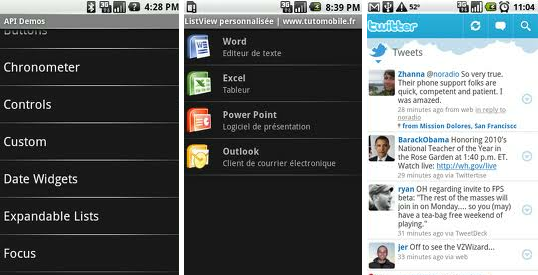
\includegraphics[width=\textwidth]{Images/Implementation/listview_example.png}
	\caption{Examples of how ListViews can be modified.}
	\label{fig:listview_example}
\end{figure}

\subsection{Benefits and Limitations}
%\textit{ Hvad er fordelen ved at bruge lister frem for at lave sin egen liste af textviews\\
%ADAPTERS\\
%Hvor langt tilbage er lister understøttet\\}
The advantage of a list view is, that we can modify the list to whatever we want it to look like without having to create any complicated programming to make it look good.
This is done by making an adapter with the layout that the items of the list is going to look like as in figure \ref{code:listview_adapter_example}, which is the adapter we use to show the children list.

\begin{figure}[H]
	\centering
		\begin{verbatim}
		View v = list_item_view;
				if (v == null) {
					LayoutInflater li = (LayoutInflater) getContext().getSystemService(
							Context.LAYOUT_INFLATER_SERVICE);
					v = li.inflate(R.layout.profile_list, null);
				}
				// FIXME: Insert pictures from admin here
				Child c = items.get(position);
				if (c != null) {
					ImageView iv = (ImageView) v.findViewById(R.id.profilePic);
					TextView tv = (TextView) v.findViewById(R.id.profileName);

					if (iv != null) {
						iv.setImageResource(R.drawable.default_profile);
					}
					if (tv != null) {
						if (c.name == "Last Used") {
							tv.setText(R.string.last_used);
						} else if (c.name == "Predefined Profiles") {
							tv.setText(R.string.predefined);
						} else {
							tv.setText(c.name);
						}
					}
				}
		\end{verbatim}
	\caption{Example of an adapter to a list view, the actual adapter used in the children list}%
	\label{code:listview_adapter_example}%
\end{figure}

Creating lists in adapters and adding adapters to list views is alot easier than making custom lists. 
Because these built in list views are very versatile and can be configured to do exactly the same as any other view in Android.\\
\\

Since lists wont be able to do anything but show a list of items without an on click listener does the list view have an interface which works exactly like any other clickable item in android.
The on click listener in the list view is as easy to implement as a button or similar clickable object.

\subsection{Lists in WOMBAT}
%\textit{ Hvordan bruger vi lister\\
%Child listen, SubProfile listen\\
%Hvordan har det indflydelse på applikationen\\}
Figure \ref{code:listview_adapter_example} is the actual implementation of the child list in WOMBAT, the only difference from the child list adapter and the configurations adapter is that the timer configurations require another text field with a description of the timer.
Which means that the configurations list only requires another layout to be constructed, which holds the extra text view.\\
\\

The on click listeners of both lists, ensures that the next fragments and Guardian object, described in \ref{??}\color[rgb]{1,0.41,0.13} REF MANGLER \color[rgb]{0,0,0}, is updated figure \ref{code:listview_onclick_example} is an example of the child fragment listview.

\begin{figure}[H]%
		\begin{verbatim}
			public void onListItemClick(ListView lv, View view, int position, long id) {
				// Update the fragments
				SubProfileFragment detf = (SubProfileFragment) getFragmentManager()
						.findFragmentById(R.id.subprofileFragment);
				CustomizeFragment custF = (CustomizeFragment)getFragmentManager().findFragmentById(R.id.customizeFragment);
				custF.setDefaultProfile();
				
				if (detf != null) {
					// Marks the selected profile in the guard singleton
					guard.profilePosition = position; 
					guard.publishList().get(position).select();
					guard.profileID = guard.publishList().get(position).getProfileId();
					detf.loadSubProfiles();
				}
			}
		\end{verbatim}
	\caption{Example of the on click listener of the child fragment}%
	\label{code:listview_onclick_example}%
\end{figure}

